\chapter{Beyond Solid-On-Solid : the Particles-Over-Particles model}
\label{chap-pop}

While Ising models describe bulk behaviour of magnetic systems \cite{niss_history_2005,niss_history_2009} but can also be used to describe interfaces between two coexisting phases \cite{abraham_interface_1976}, a direct interface lattice models exists, which is called Solid-On-Solid. This model was first studied by Gilmer and Bennema \cite{gilmer_computer_1972,gilmer_simulation_1972} as a way to compute the crystal growth, whose dynamical equation will be later known as the Edwards-Wilkinson equation \cite{edwards_surface_1982,halpin-healy_kinetic_1995} . In a second time, correspondance between SOS and the highly anisotropic Ising model at low temperature where found \cite{swendsen_roughening_1977,guyer_sine-gordon_1979}, with the exact derivation of the SOS hamiltonian from the Ising one explained in Sec \ref{sec-sos}. When using an exponent of 2 in the interaction between nearest sites, the Gaussian SOS exhibits similar behavior to fluid interfaces \cite{muller-krumbhaar_kinetic_1976,baillie_solid_1993}.
In Monte Carlo simulations for the Ising model, spins are taken with a uniform probability \cite{metropolis_monte_1949,newman_monte_1999}, which allows the study of interface dynamics \cite{schmittmann_driven_1998,muller_profile_2005,smith_interfaces_2008-1,smith_lateral_2010}. On the contrary in the SOS aproximation it is the heights which are taken with a uniform probability \cite{wilby_scaling_1992,siegert_scaling_1993} thus discarding bulk information. 

Driven by this lack of correspondence between both models, in this chapter we modernize Temperley's model \cite{temperley_statistical_1952} with a model that we call {\bf Particles-Over-Particles} which takes into account combinatorial terms, giving rise to an entropic contribution.
By noticing that the height $h$ of the interface is the sum of all particles of size $a=1$ which are put under it, we first develop the partition function and transfer matrix of our model and compare it to Ising and SOS (to our knowledge there has been no direct comparison between Ising and SOS in literature), then we develop the M-particles system where we introduce multiple types of particles stacked vertically, where each type may obey to a different dynamic, kinetic coefficient or diffusive constant.

%%%%%%%%%%%%%%%%%
\section{The model}
%%%%%%%%%%%%%%%%%

In a SOS system of size $L'$ , the height of the interface at site $i$ is noted $h_i \in [0,L]$ at site $i$, and fixing the total number of particles to be N the partition function is given by
\begin{align}
Z_{SOS}(N) = \sum_{h_0 h_1 ... h_{L'}} \delta_{\sum_i h_i, N} \exp\left(-\beta J \sum_{i=1}^{L'} |h_{i+1}-h_i| -\beta B\sum_{i=1}^{L'} V(h_i)\right)
\end{align}
where $V(h)$ is a function of the internal variables $h_i$ and $B$ the coupling parameter which has the dimension of energy. As we do in the case of a perfect gas, if the height profiles represent particle numbers which are all identical, the partition function is given by
\begin{equation}
Z_{POP}(N) = \frac{1}{N!}\sum_{h_1,h_2\cdots h_{L'}} \delta_{\sum_{i=1}^{L'} h_i, N}\frac{N!}{\prod_{i=1}^{L'} h_i!} \exp\left(-\beta J \sum_{i=1}^{L'} |h_{i+1}-h_i| -\beta B \sum_{i=1}^{L'} V(h_i)\right)
\end{equation}
Here the combinatorial term $\frac{N!}{\prod_{i=1}^L h_i!}$ represents the number of ways that the $h_i$ particles on each site can be chosen from the $N$ particles available. In the same fashion as the Solid-On-Molid, we call this model the \textbf{Particles-Over-Particles model}, since we stack particles in columns of height $h_i$. The constraint on the particle number makes the computation of the partition function at fixed $N$ complicated both analytically and numerically. However, if we change to the grand canonical ensemble using
the formula
\begin{equation}
\Xi = \sum_{N} \exp(\beta\mu N) Z_{POP}(N)
\end{equation}
where $\Xi$ is the grand partition function and $\mu$ the chemical potential, we find
\begin{equation}
\Xi_{POP} = \sum_{h_1,h_2\cdots h_{L'}} \frac{1}{\prod_{i=1}^{L'} h_i!} \exp\left(-\beta J \sum_{i=1}^{L'} |h_{i+1}-h_i| -\beta B \sum_{i=1}^{L'}[ V(h_i)-\mu h_i]\right)
\end{equation}
The model differs from the usual solid on solid model in that a number of particle configurations give rise to the same height configurations. The grand partition function can then be written as 
\begin{equation}
\Xi = \sum_{h_1,h_2\cdots h_{L'}} \exp\left(-\beta H_{eff}(h_1,h_2\cdots h_{L'})\right)
\end{equation}
where 
\begin{equation}
H_{eff}= J \sum_{i=1}^{L'} |h_{i+1}-h_i| +\sum_{i=1}^{L'} [B V(h_i)-\mu h_i +\frac{1}{\beta}\ln(h_i !)]
\label{heff-pop}
\end{equation}

\begin{figure}
\centering
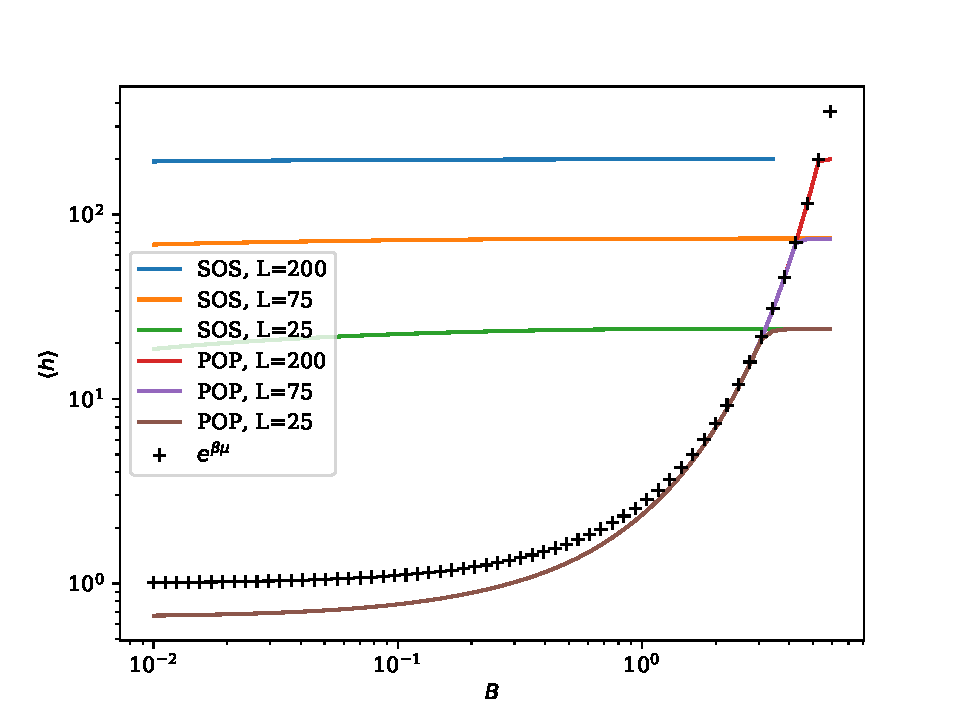
\includegraphics{pop/hauteur-tm-pop-sos.pdf}
\caption{Mean height of the SOS (for reference) and POP model with respect the chemical potential $\mu$ through transfer matrix with different maximal heights in the thermodynamic limit $L'\to \infty$, compared to the Striling's approximation Eq \eqref{stirling-pop},at $\beta=1$. }
\label{haut-tm-pop} 
%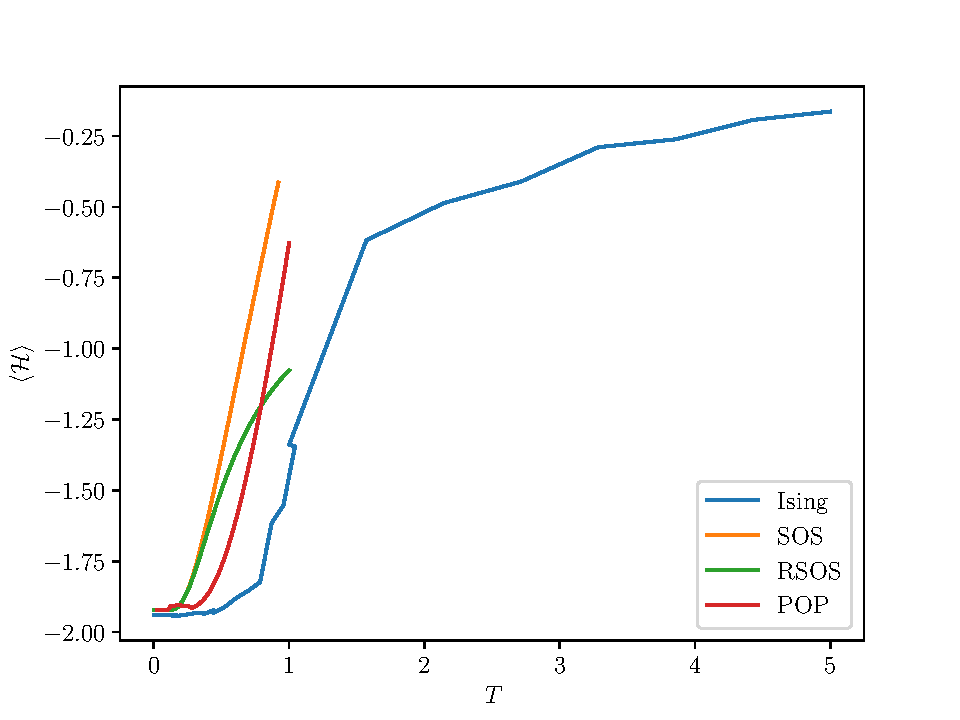
\includegraphics{pop/comparaison-modeles.pdf}
%\caption{Comparison of the internal mean total energy of the Ising, SOS, RSOS and POP models with respect to temperature in absence of external field and $\mu=0$, from Monte Carlo simulations at $L'=126$ and $L=30$ with Glauber dynamics. We used Eq \ref{energie-sos-ising} to compare energies between the interface models and the Ising one.
%{\color{red} redo sims for Ising, need MCIA, takes too long otherwise}}
%\label{comp-models}
\end{figure}

The transfer matrix is
\begin{align}
T_{POP}(h,h') = T_{SOS}(h,h') \exp \left(- \frac{\ln(h)+\ln(h')}{2} \right)
\end{align}

Contrary to the SOS model where there needs to be a confining external field in order to localize the interface \cite{burkhardt_localisation-delocalisation_1981,chui_pinning_1981}, the entropic term gives a stable position for the interface. In absence of external field $B=0$, the effective potential is given by
\begin{align} 
    V_{eff}(h) = - \mu h + \frac{1}{\beta}\ln(h!)
\end{align}
If the chemical potential is large enough, the number of particles $N$ is large enough, so we can use Striling's formula and approximate a continuous derivative with the finite-difference in $h$, so we have
\begin{align} 
    V_{eff}(h)' = - \mu +\frac{1}{\beta} \ln(h)
\end{align}which gives the mean height 
\begin{align} 
    <h> = \exp(\beta \mu) 
\label{stirling-pop}
    \end{align}
    In Fig \ref{haut-tm-pop}, we show the mean height \eqref{stirling-pop} compared to the transfer matrix diagonalisation with different matrix size and the Monte Carlo simulations at $\beta=1$. We see that when $ <h> \gg 1$, the Stirling's formula becomes valid and Eq \eqref{stirling-pop} becomes accurate. Since $<h>$ cannot exceed the maximum size of the system, saturation occurs at large $\mu$. SOS mean height is also plotted as a reference, where we see that even in the limit $\mu=0$, the mean height is equal to $<h>(\mu=0) = \frac{L}{2}$.

The Kawasaki implementation is straightforward, we choose a particle $n$ with probability $\frac{1}{N}$ at each Monte Carlo step, then we attempt to move the particle to the left or right using Metropolis acceptance rate.

The Glauber case is trickier. At equilibrium, we expect that as many particles are added as subtracted, so we attempt with probability $0.5$ to add a particle, and to remove one with the same probability. When adding a particle, we choose a site $i$ with uniform probability $1/L'$, so the selection rate is 
\begin{align}
g(h_i \to h_i+1) = \frac{1}{2L'}
\end{align}
To remove a particle \footnote{In C++, we can use a $std::vector$ in which we add or remove particles. After each success attempt, we rebuild the distribution $std::uniform\_int\_distribution(0,N-1)$, where N is the number of particles. This operation is lightweight and should not cause any slowing down. For the next section's algorithm with multiple particle types, we use $std::discrete\_distribution<>$. }, we choose a particle $n$ with uniform probability $1/N$, meaning that the selection probability is 
\begin{align}
g(h_i \to h_i-1) = \frac{h_i}{2N}
\end{align}
In the case that there is no particle in the system, we skip that phase and we immediately proceed to attempt to add a new particle.
In order to satisfy detailed balance, we thus need acceptance rates such that verify
\begin{align}
\frac{g(h_i \to h_i+1)}{g(h_i+1 \to h_i)} \frac{A(h_i \to h_i+1)}{A(h_i \to h_i+1)}
=& \frac{N}{L' (h_i+1)} \frac{A(h_i \to h_i+1)}{A(h_i \to h_i+1)} \nn
=& \exp(-\beta (E(h_i+1)-E(h_i)) 
\end{align}
Choosing an acceptance rate that satisfies this condition is not as easy as the Metropolis acceptance rate \cite{metropolis_monte_1949}, and we provide no clear answer as to how solve this problem. Using the Metropolis acceptance rate ($A(\mu \to \nu) = 1$ if $\Delta_E < 0$) does not to provide the correct equilibrium averages expected by the transfer matrix.

Here, the combinatoric term is directly taken into account in the selection probability, which is why it is difficult to find a good acceptance rate. Nevertheless, it is possible to use uniform selection probability as with SOS and introduce the combinatoric term in the energy. 
%In Fig \ref{comp-models}, we plot the internal energy of the Ising, SOS, RSOS and POP models with respect to temperature in absence of external fields and $\mu=0$ wtih non-conserved dynamics. {\color{red} discuss the graph once plots are better}

%%%%%%%%%%%%%%%%%%%%
\section{$M$-particles POP system}
%%%%%%%%%%%%%%%%%%%%

\begin{figure}
\centering
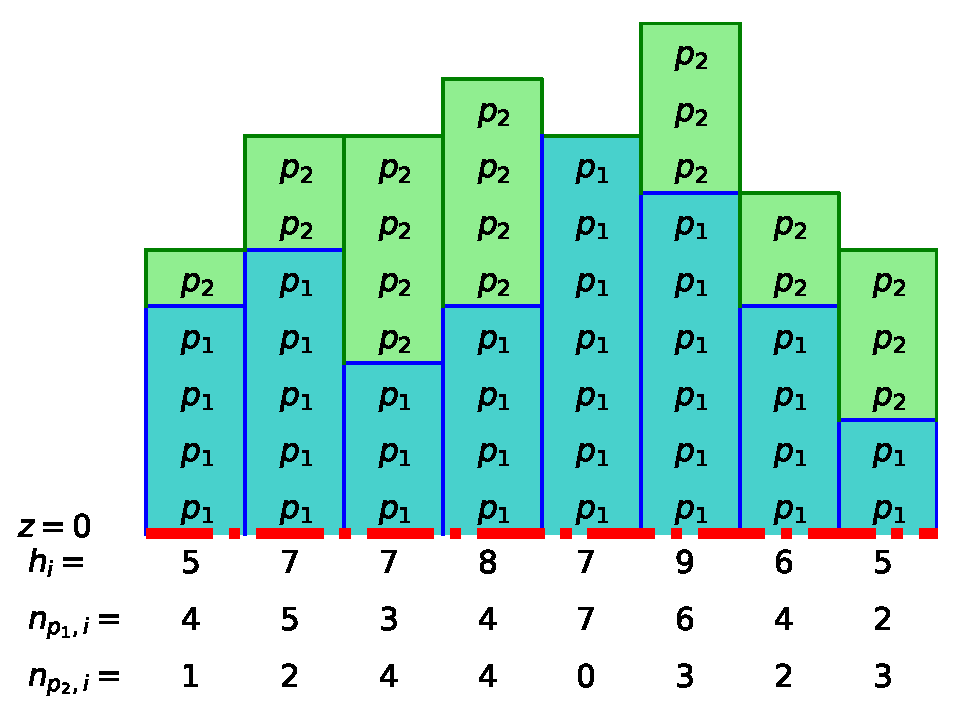
\includegraphics[width=0.7\linewidth]{pop/figure-pop.pdf}
\caption{Possible POP configuration with two types of particles $p_1$ and $p_2$. The red line shows the origin $z=0$. In the $i$-th column the interface is at height $h_i$, with $n_{1,i}$ particles of type $p_1$ at site $i$, and same for particles $p_2$. Over the interface, there are no particles. }
\label{fig-pop}
\end{figure}

The Ising model with spins $\sigma= \pm1$ has a direct mapping with liquid/gas and binary mixtures systems \cite{goldenfeld_lectures_2018}, which are systems with two types of particles (for the liquid/gas model we can say that $\sigma$ is a "density particle"). On the contrary, SOS models only need the existence of one type of particles, since everything that is over the interface is not taken into account. We can immagine multi-layering of non-miscible liquids having different densities \cite{wang_instability_1978,bonizzi_simulation_2003}, forming many layers with $M-1$ interfaces, $M$ being the number of particles type. We can decide to study one specific interface between two particle types, and in such case the classic SOS model would be enough, with $J$ being the surface tension between both liquids. 

In this multi-layered system, we consider a model of a surface delimiting a bulk phase of $L'$ sites which contains $M$ different particle types $p_1 ... p_M$, $N_m$ is the total number of particles of type $m$ and $n_{m,i}$ denotes the number of particles of type $m$ at site $i$. The interface height is $h_i = \sum_m n_{m,i}$. Taking into account the entropic contribution, the effective Hamiltonian for the model is
\begin{align}
H[M] = J \sum_i |h_i-h_{i+1}| + B \sum_i V(h_i) - \sum_m \mu_m \sum_i n_{m,i} + \frac{1}{\beta} \sum_m \sum_i \ln(n_{m,i})
\label{ham-pop-c}
\end{align}
We assume that the particles in each column are demixed, i.e. the permitted particle configurations are taken to be stacked vertically such that the stack of $p_{m+1}$ particles lies on top of the $p_m$ particles, as seen in Fig \ref{fig-pop} for $M=2$. The first term in the Hamiltonian corresponds to the surface tension with a gas phase above the stacks of particles. As discused with the SOS model, we can have a restricted or gaussian version of Eq \ref{ham-pop-c}. 

The grand partition function is given by
\begin{align}
\Xi = \sum_{{\bf n_1...n_M}} \exp(-\beta H[M])
\end{align}

If $M=2$, the the statics of the above can be reduced to the study of a single particle model by making the change of variable $n_{2,i} = h_i - n_{1,i}$. Using the binomial relation ${(a+b)^{n_1} = \sum_{h'=0}^h \frac{h!}{h'! (h-h')!} a^{h'} b^{h'-h}}$, the sum over the variables $n_{1,i}$ can be trivially carried out and we find
\begin{align}
\Xi =& \sum_{\bf h} \exp \left( -\beta J \sum_i |h_i-h_{i+1}| - \beta B \sum_i V(h_i) - \sum_i \ln(h_i!) + \beta \mu_e \sum_i h_i \right) \nn
=& \sum_{\bf h} \exp \left( -\beta H_{eff}(h_1,h_2...h_{L'}) \right)
\end{align}
where $\mu_e = \frac{1}{\beta}\ln( \exp(\beta \mu_1) + \exp(\beta \mu_2)$ is the effective chemical potential for the variables $h_i$. If we add a third type of particle, we clearly see that the same reduction can be carried out. Thus, by recursivity, we can show that for any number of particle type $M$, we have the same effective Hamiltonian as the single particle system \eqref{heff-pop}, with an effective chemical potential
\begin{align}
\mu_e = \frac{1}{\beta} \ln \left( \sum_m \exp( \beta \mu_m ) \right)
\end{align}
An interesting thing to remark is that even if the chemical potential of a particle type $\mu_m = 0$, its contribution to the effective chemical potential is nonzero. 
This reduced theory can be numerically solved in equilibrium by transfer matrix methods. 

Now let the subset $\bar{M}$ of particle types from the $M$ particle types be in the canonical ensemble, while all the other ones are in the grand-canonical one. This is the so-called model C \cite{hohenberg_theory_1977}, which describes the coupling between conserved and non-conserved fields, such as impurities in liquids \cite{crisanti_dynamics_1992} or ionic conductors moving through a lattice set up by different types of ions \cite{dieterich_theoretical_1980,katz_nonequilibrium_1984}.
The total partition function is then
\begin{align}
\Xi = \sum_h \exp \left( -\beta H_{eff}(h_1,h_2...h_{L'}) \right) \prod_{m \in \bar{M}} \delta_{\sum_{i=1}^{L'} h_i,N_m}
\end{align}
with the average number of particles per site being
\begin{align}
< n_m > =& \frac{1}{\beta L'} \frac{\partial}{\partial \mu_m} \ln(\Xi) \nn
=& \frac{1}{\beta L'} \frac{\partial \mu_e}{\partial \mu_m} \frac{\partial}{\partial \mu_e} \ln(\Xi) \nn
=& \frac{\exp(\beta \mu_m)}{\sum_m \exp(\beta \mu_m)} 
\end{align}
where $ = <\sum_m n_m>$. 


Mixing Glauber and Kawasaki dynamics for different particle types could be implemented using the following algorithm. Each non-conserved particle type possess a kinetic coefficient $\alpha_m$, while each conserved particle type has a diffusive coefficient $D_m$. We set $p_m = \alpha_m$ if the particle is non-conserved, and $p_m = D_m$ otherwise, and we normalize it in order to have $\sum_m p_m = 1$. At each Monte Carlo step, a particle of type $m$ is chosen with probability $p_m$, and then we proceed with Glauber or Kawasaki dynamics for a single-type particle system, as described in the previous section.
To satisfy detailed balance, we have to understand how this coefficient $p_m$ changes the selection probability $g$, and we get the same difficulties as in the single-particle type Glauber case.

Nevertheless, when all particles are under Kawasaki dynamics and $p_m = 1/M$ is a constant, then the ratio between selection rates is equal, which solves all the issues. 

This algorithm could prove useful for studying multi-particle systems where each particle type is under different potentials (think of an ion in a neutral solvent under magnetic field) or different temperature \cite{grosberg_nonequilibrium_2015}, some of them which are under non-equilibrium forces like shearing.


%%%%%%%%%%%%%%%%%%%%%%
\section{Continuum Theory} 
%%%%%%%%%%%%%%%%%%%%%%

In order to understand the statics of the model we write a continuum version of the theory with $M$ field $n_m(x)$ and we take the a Gaussian form for the surface energy
\begin{equation}
H = \int dx \frac{\sigma}{2} [\frac{d}{dx} (\sum_m n_m)]^2 + V(n_1(x),...,n_M(x))
\end{equation}
where $\sigma$ is the surface tension and 
\begin{equation}
V(n_1(x),...n_M(x)) = \sum_m -\mu_m n_m(x) + T n_m(x) [ \ln(n_m(x))-1 ]
\end{equation}
We have used Stirlings formula and thus assumed that the typical value of $n_m(x)$ aree large. 
We now expand $V(n_1(x),...n_M(x))$ by writing $n_m(x) = \overline n_m + \phi_m(x)$ where $(\overline n_1,..\overline n_M)$ is the minimum of $V(n_1,..n_M)$. Here we find
\begin{equation}
\overline n_m = \exp(\beta \mu_m) 
\end{equation}

This gives an effective Hamiltonian for the fluctuations of the fiels $\phi_m$ 
\begin{equation}
H_f = \frac{\sigma}{2}\int dx [\frac{d}{dx}(\sum_m \phi_m]^2 + \sum_m r_m \phi_m^2(x) 
\end{equation}
where 
\begin{equation}
r_m = \frac{T}{\sigma \overline n_m} \
\end{equation}
A straight-forward calculation then shows that the Fourier transform of the connected height-height fluctuation correlation function is
\begin{equation}
\tilde C_{hh}(k) = \frac{T}{\sigma} \frac{1}{k^2 + r_e}
\label{stat}
\end{equation}
where $r_e = \prod_m r_m/ \sum_m r_m$. We thus find
\begin{equation}
= \frac{T}{2\sigma m_e} = \frac{1}{2}\sqrt{\frac{T\overline h}{\sigma}},
\end{equation}
where $\overline h= \sum_m \overline n_m$.

%%%%%%%%%%%%%%%
\section{Conclusion}
%%%%%%%%%%%%%%%

There are two ways of interpreting the interface's description thought its height $\{h_i\}$. The first one is to only see the height as the interface's degrees of freedom \cite{gilmer_computer_1972,gilmer_simulation_1972}, while the second one is to interpret that height as a number of particles of type A which are below the interface with particles of type B, which is the physical phenomenon happening in crystal growth. This interpretation requires the addition of an entropic term \cite{temperley_statistical_1952}, which localises the free interface in a semi-infinite geometry, contrary to SOS models \cite{chui_pinning_1981}. The system can also be composed of multiple layers of different particles [multilayer], and this new model can take that into account for numerical simulations. 
The problem lies in the numerical algorithm. Taking a height with non-uniform probability is tricky, as it changes the selection probability $g(C\to C')$, so the acceptance probability $A(C\to C')$ is not as simple as the Metropolis one \cite{metropolis_monte_1949,newman_monte_1999}. We let the resolution of this problem - and as such the study of new physics through numerical simulations of this model - to the community. 